\chapter{Structure from Motion}
通过相机运动重建物体.

Problems tobe noticed
\begin{enumerate}
    \item How the camera maps the 3D points in the world onto its image plane. (camera model)(如何把三维坐标映射为二维坐标)
    \item How tocompute the position and orientation of the camera w.r.t. the world coordinate frame. (camera calibration and pose estimation)(如何恢复相机参数,位姿)
    \item How to reconstruct the unknown 3D structure from images.  (structure from motion)(恢复场景)
\end{enumerate}

\section{Camera model}
几何变换
\subsection{Image Formation}
\begin{enumerate}
    \item 相机定位 (Coordinate Transformation, 坐标变换, 从世界坐标系到相机坐标系)
    \item 快门 (Perspective Projection, 透视投影变换)
    \item 图像形成 (Image Plane to Image Sensor Mapping, 从物理坐标到像素坐标)
\end{enumerate}

\begin{itemize}
    \item Extrinsic Matrix(外参): Coordinate Transformation
    \item Intrinsic Matrix(内参): Perspective Projection + Image Plane to Image Sensor Mapping
\end{itemize}

\subsubsection{Coordinate Transformation}
\begin{figure}[H]
    \centering
    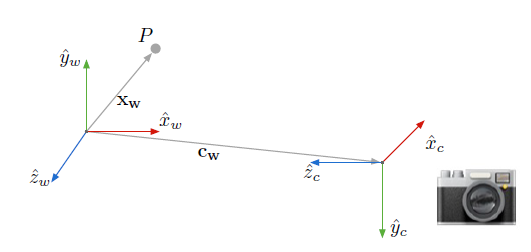
\includegraphics[width=0.58\textwidth]{Lec7/Coordinate Transformation}
    \caption{Coordinate Transformation}
\end{figure}
\begin{align*}
    x_w=\begin{bmatrix}
        x_w\\y_w\\z_w
    \end{bmatrix} \Longrightarrow x_c=\begin{bmatrix}
        x_c\\y_c\\z_c
    \end{bmatrix}
\end{align*}

需要知道相机位置与朝向(位姿). Position $c_w$为世界中心到相机中心的向量, Orientation $R$为旋转矩阵, 且$R$为正交矩阵. 
\begin{align*}
    R=\begin{bmatrix}
        r_{11} & r_{12} & r_{13} \\
        r_{21} & r_{22} & r_{23} \\
        r_{31} & r_{32} & r_{33}
    \end{bmatrix}\begin{matrix}
        \longrightarrow \text { Row 1: Direction of } \hat{x}_{c} \text { in world coordinate frame }\\
        \longrightarrow \text { Row 2: Direction of } \hat{y}_{c} \text { in world coordinate frame }\\
        \longrightarrow \text { Row 3: Direction of } \hat{z}_{c} \text { in world coordinate frame }
    \end{matrix}
\end{align*}

现在对一世界坐标P, 其坐标为$x_w$, 有: (即旋转后平移一下)
\begin{align*}
    x_c&=R(x_w-c_x)=Rx_w+t\\
    t&=-Rc_w
\end{align*}
\begin{align*}
    x_c=\begin{bmatrix}
        x_c\\y_c\\z_c\\
    \end{bmatrix}=\begin{bmatrix}
        r_{11} & r_{12} & r_{13} \\
        r_{21} & r_{22} & r_{23} \\
        r_{31} & r_{32} & r_{33}
    \end{bmatrix}\begin{bmatrix}
        x_w\\y_w\\z_w
    \end{bmatrix}+\begin{bmatrix}
        t_x\\t_y\\t_z
    \end{bmatrix}
\end{align*}
\begin{align*}
    \tilde{x}_c=\begin{bmatrix}
        x_c\\y_c\\z_c\\1
    \end{bmatrix}&=\begin{bmatrix}
        r_{11} & r_{12} & r_{13} & t_x\\
        r_{21} & r_{22} & r_{23} & t_y\\
        r_{31} & r_{32} & r_{33} & t_z\\
        0&0&0&1
    \end{bmatrix}\begin{bmatrix}
        x_w\\y_w\\z_w\\1
    \end{bmatrix}\\
    \therefore \,  \text{外参矩阵 } M_{ext}&=\begin{bmatrix}
        R_{3\times 3}&\mathrm{t}\\
        \mathrm{0}_{1\times 3}&1
    \end{bmatrix}=\begin{bmatrix}
        r_{11} & r_{12} & r_{13} & t_x\\
        r_{21} & r_{22} & r_{23} & t_y\\
        r_{31} & r_{32} & r_{33} & t_z\\
        0&0&0&1
    \end{bmatrix}
\end{align*}

\subsubsection{Perspective Projection}
\begin{figure}[H]
    \centering
    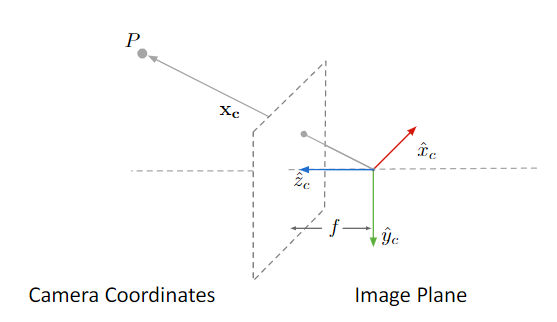
\includegraphics[width=0.58\textwidth]{Lec7/Perspective Projection }
    \caption{Perspective Projection }
\end{figure}
\begin{align*}
    x_c=\begin{bmatrix}
        x_c\\y_c\\z_c
    \end{bmatrix}\Longrightarrow x_i=f\cdot \begin{bmatrix}
        \frac{x_c}{z_c}\\ \frac{y_c}{z_c} \\1
    \end{bmatrix}
\end{align*}

\subsubsection{Image Plane to Image Sensor Mapping}
从毫米坐标变为像素坐标. 需要分辨率. 

\begin{figure}[H]
    \centering
    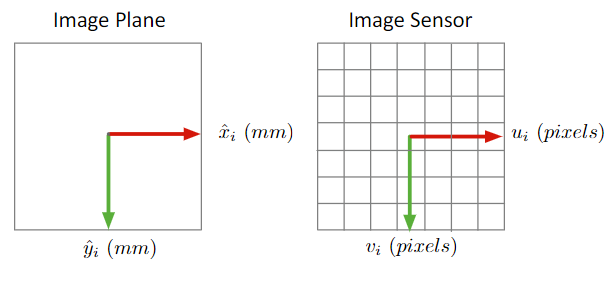
\includegraphics[width=0.58\textwidth]{Lec7/Image Plane to Image Sensor Mapping}
    \caption{Image Plane to Image Sensor Mapping}
\end{figure}

$m_x$与$m_y$为方向上的分辨率. 
\begin{align*}
    u&=m_x x_i= m_x f \frac{x_c}{z_c}\\
    v&=m_y y_i= m_y f \frac{y_c}{z_c}
\end{align*}

\begin{figure}[H]
    \centering
    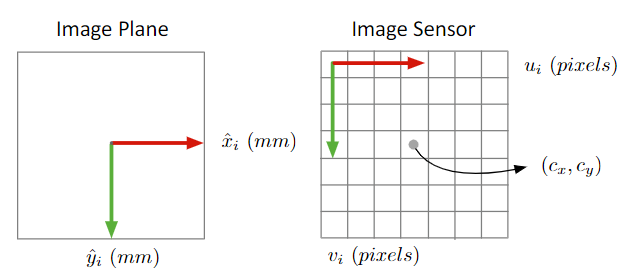
\includegraphics[width=0.58\textwidth]{Lec7/Principle Point}
    \caption{Principle Point}
\end{figure}

但二者原点不一样, 需要有偏移量 $(c_x,c_y)$(一般情况是图像中心, 但如果图像被裁切过, 图像中心会改变)
\begin{align*}
    u&= m_x f \frac{x_c}{z_c}+c_x\\
    v&= m_y f \frac{y_c}{z_c}+c_y
\end{align*}

综上所述, (令$f_x=m_xf, f_y=m_yf$)
\begin{align*}
    \begin{bmatrix}
        u\\v\\1
    \end{bmatrix}\equiv\begin{bmatrix}
        u\\v\\w
    \end{bmatrix}&=\begin{bmatrix}
        f_x & 0 & c_x & 0\\
        0&f_y&c_y&0\\
        0&0&1&0
    \end{bmatrix}\begin{bmatrix}
        x_c\\y_c\\z_c\\1
    \end{bmatrix}\\
    \therefore \,  \text{内参矩阵 } M_{int}&=\begin{bmatrix}
        f_x & 0 & c_x & 0\\
        0&f_y&c_y&0\\
        0&0&1&0
    \end{bmatrix}
\end{align*}

\subsection{Projection Matrix P}
再综上所述, 最终的投影矩阵P: 
\begin{align*}
    \tilde{x}_c&=M_{ext}\tilde{x}_w \text{  World toCamera}\\
    \tilde{u}&=M_{int}\tilde{x}_c \text{  Camera to Pixel}\\
    \therefore \,  \tilde{u}&=M_{int}M_{ext}\tilde{x}_w=P\tilde{x}_w\\
    \begin{bmatrix}
        u\\
        v\\
        w\\
    \end{bmatrix}&=\begin{bmatrix}
        p_{11} & p_{12} & p_{13} & p_{14} \\
        p_{21} & p_{22} & p_{23} & p_{24} \\
        p_{31} & p_{32} & p_{33} & p_{34}
    \end{bmatrix}\begin{bmatrix}
        x_w\\y_w\\z_w\\1
    \end{bmatrix}
\end{align*}

\section{Camera calibration}
相机标定
\subsection{Camera Calibration Procedure}
\begin{enumerate}
    \item Capture an image of an object with known geometry. (拍摄一已知物体, 已知角点世界坐标)
    \item Identify correspondences between 3D scene points and image points. (检测与匹配, 得到角点在图像中二维坐标) 
    \begin{figure}[H]
        \centering
        \begin{minipage}{0.38\textwidth}
            \centering
            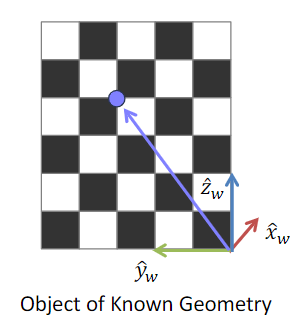
\includegraphics[width=\textwidth]{Lec7/known geometry}
            \caption{标定板}
        \end{minipage}
        \begin{minipage}{0.38\textwidth}
            \centering
            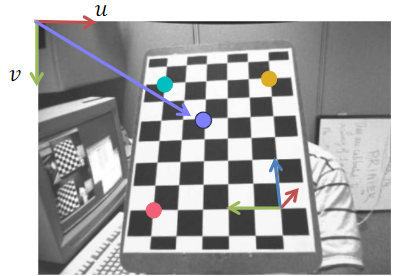
\includegraphics[width=\textwidth]{Lec7/Captured Image}
            \caption{拍照}
        \end{minipage}
    \end{figure}
    \item For each corresponding point $i$ in scene and image (从已知坐标求解投影矩阵P)
    
    \begin{align*}
        \begin{bmatrix}
            u^{(i)}\\
            v^{(i)}\\
            w^{(i)}\\
        \end{bmatrix}&\equiv\begin{bmatrix}
            p_{11} & p_{12} & p_{13} & p_{14} \\
            p_{21} & p_{22} & p_{23} & p_{24} \\
            p_{31} & p_{32} & p_{33} & p_{34}
        \end{bmatrix}\begin{bmatrix}
            x_w^{(i)}\\y_w^{(i)}\\z_w^{(i)}\\1
        \end{bmatrix}\\
        u^{(i)}&=\frac{p_{11} x_{w}^{(i)}+p_{12} y_{w}^{(i)}+p_{13} z_{w}^{(i)}+p_{14}}{p_{31} x_{w}^{(i)}+p_{32} y_{w}^{(i)}+p_{33} z_{w}^{(i)}+p_{34}} \\
        v^{(i)}&=\frac{p_{21} x_{w}^{(i)}+p_{22} y_{w}^{(i)}+p_{23} z_{w}^{(i)}+p_{24}}{p_{31} x_{w}^{(i)}+p_{32} y_{w}^{(i)}+p_{33} z_{w}^{(i)}+p_{34}}
    \end{align*}

    \item Rearranging the terms(最少6组)
    \addtocounter{MaxMatrixCols}{15}
    \begin{align*}
        \begin{array}{cccc}
            \begin{bmatrix}
            x_{w}^{(1)} & y_{w}^{(1)} & z_{w}^{(1)} & 1 & 0 & 0 & 0 & 0 & -u_{1} x_{w}^{(1)} & -u_{1} y_{w}^{(1)} & -u_{1} z_{w}^{(1)} & -u_{1} \\
            0 & 0 & 0 & 0 & x_{w}^{(1)} & y_{w}^{(1)} & z_{w}^{(1)} & 1 & -v_{1} x_{w}^{(1)} & -v_{1} y_{w}^{(1)} & -v_{1} z_{w}^{(1)} & -v_{1} \\
            \vdots & \vdots & \vdots & \vdots & \vdots & \vdots & \vdots & \vdots & \vdots & \vdots & \vdots & \vdots \\
            x_{w}^{(i)} & y_{w}^{(i)} & z_{w}^{(i)} & 1 & 0 & 0 & 0 & 0 & -u_{i} x_{w}^{(i)} & -u_{i} y_{w}^{(i)} & -u_{i} z_{w}^{(i)} & -u_{i} \\
            0 & 0 & 0 & 0 & x_{w}^{(i)} & y_{w}^{(i)} & z_{w}^{(i)} & 1 & -v_{i} x_{w}^{(i)} & -v_{i} y_{w}^{(i)} & -v_{i} z_{w}^{(i)} & -v_{i} \\
            \vdots & \vdots & \vdots & \vdots & \vdots & \vdots & \vdots & \vdots & \vdots & \vdots & \vdots & \vdots \\
            x_{w}^{(n)} & y_{w}^{(n)} & z_{w}^{(n)} & 1 & 0 & 0 & 0 & 0 & -u_{n} x_{w}^{(n)} & -u_{n} y_{w}^{(n)} & -u_{n} z_{w}^{(n)} & -u_{n} \\
            0 & 0 & 0 & 0 & x_{w}^{(n)} & y_{w}^{(n)} & z_{w}^{(n)} & 1 & -v_{n} x_{w}^{(n)} & -v_{n} y_{w}^{(n)} & -v_{n} z_{w}^{(n)} & -v_{n}
            \end{bmatrix} &
            \begin{bmatrix}
                p_{11}\\ p_{12} \\p_{13}\\p_{14}\\p_{21}\\p_{22}\\p_{23}\\p_{24}\\p_{31}\\p_{32}\\p_{33}\\p_{34}
            \end{bmatrix}
            &=&\begin{bmatrix}
                0\\0\\0\\0\\
                0\\0\\0\\0\\
                0\\0\\0\\0\\
            \end{bmatrix}\\
            A&\vec{p}&\\
            \text{Known} &\text{Unknown}&
        \end{array}
    \end{align*}
    \addtocounter{MaxMatrixCols}{10}
    \item Solve for $p$
    \begin{align*}
        A\vec{p}=0
    \end{align*}
\end{enumerate}

\subsection{Property of Projection Matrices: Scale}
投影矩阵$P$仅按尺度定义, 即哪怕知道了物体与相片的具体对应, 相机的参数仍有无穷多种解. 例如只要视场角相同, 不同焦距配上合适距离可以拍摄出一致的图像. 

\begin{align*}
    \begin{bmatrix}
        \tilde{u}\\\tilde{v}\\\tilde{w}
    \end{bmatrix}\equiv k\begin{bmatrix}
        \tilde{u}\\\tilde{v}\\\tilde{w}
    \end{bmatrix},\quad k\ne 0
\end{align*}
\begin{align*}
    \therefore \,  P\equiv kP
\end{align*}

所以需要一定约束. 
\begin{itemize}
    \item Option 1: $p_{34}=1$
    \item Option 2: $\left\| \vec{p} \right\|^2=1$, 一般用此
\end{itemize}

求为
\begin{align*}
    \min_{\vec{p}} \left\| A\vec{p} \right\|^2 ,\text{ when} \left\| \vec{p} \right\|=1
\end{align*}

可以证明$A^T A$最小特征值$\lambda$对应的特征向量为最优的$\vec{p}$, 然后通过$\vec{p}$重构出$P$. 

\subsection{Decompose Projection Matrices to Intrinsic and Extrinsic Matrices}
将$P$分解为内参矩阵与外参矩阵. 

\begin{align*}
    \begin{array}{cccccc}
        P&=&\begin{bmatrix}
            p_{11} & p_{12} & p_{13} & p_{14} \\
            p_{21} & p_{22} & p_{23} & p_{24} \\
            p_{31} & p_{32} & p_{33} & p_{34}
        \end{bmatrix}&=&\begin{bmatrix}
            f_x & 0 & c_x & 0\\
            0&f_y&c_y&0\\
            0&0&1&0
        \end{bmatrix}&\begin{bmatrix}
            r_{11} & r_{12} & r_{13} & t_x\\
            r_{21} & r_{22} & r_{23} & t_y\\
            r_{31} & r_{32} & r_{33} & t_z\\
            0&0&0&1
        \end{bmatrix}\\
         & & & &M_{int}&M_{ext} 
    \end{array}
\end{align*}

K 为上三角矩阵, R为正交矩阵, 可以通过``QR factorization''从KR分解出唯一的K与R. 
\begin{align*}
    \begin{bmatrix}
        p_{11} & p_{12} & p_{13}\\
        p_{21} & p_{22} & p_{23}\\
        p_{31} & p_{32} & p_{33}\\
    \end{bmatrix}=\begin{bmatrix}
        f_x &0&c_x\\
        0&f_y&c_y\\
        0&0&1&
    \end{bmatrix}\begin{bmatrix}
        r_{11} & r_{12} & r_{13}\\
        r_{21} & r_{22} & r_{23}\\
        r_{31} & r_{32} & r_{33}
    \end{bmatrix}=KR
\end{align*}

然后有
\begin{align*}
    \begin{bmatrix}
        p_{14} \\
        p_{24} \\
        p_{34}
    \end{bmatrix}=\begin{bmatrix}
        f_x &0&c_x\\
        0&f_y&c_y\\
        0&0&1&
    \end{bmatrix}\begin{bmatrix}
        t_x\\
        t_y\\
        t_z\\
    \end{bmatrix}=K\vec{t}
\end{align*}
\begin{align*}
    \therefore \,  \vec{t}=K^{-1}\begin{bmatrix}
        p_{14} \\
        p_{24} \\
        p_{34}
    \end{bmatrix}
\end{align*}

\subsection{Camera Distortions}
相机会因为镜头有非透视投影导致的畸变, 这些畸变可以被公式描述, 得到畸变参数后, 也可以通过优化消除. 但这里忽略了. 

\subsection{Visual Locaization Problem}
视觉定位问题(求解外参, 默认内参已知)

\begin{enumerate}
    \item 找到对应关系 (3D-2D): 同样通过图像匹配
    \item 已知3D世界坐标与对应2D相机坐标后求解外参(一般假设内参已知) 
\end{enumerate}

\begin{figure}[H]
    \centering
    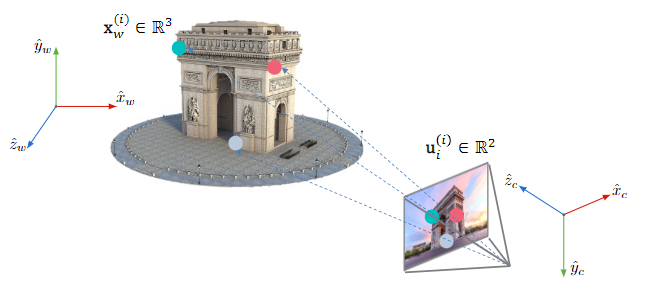
\includegraphics[width=0.68\textwidth]{Lec7/3D-2D}
    \caption{3D-2D}
\end{figure}

\subsection{Perspective-n-Point problem(PnP)}
给定三维点坐标与对应图像的位置, 求解相机的位置与旋转. 

旋转矩阵虽然是3x3但只有三个角度参数, 再加上三个平移参数, 统共为6自由度, 所以问题也称6DoF

\subsubsection{Direct Linear Transform (DLT)}
直接硬解, 但不常用, 因为内参已知
\begin{align*}
    \begin{array}{cccc}
        \begin{bmatrix}
            u^{(i)}\\v^{(i)}\\1
        \end{bmatrix}&\equiv&\begin{bmatrix}
            p_{11} & p_{12} & p_{13} & p_{14} \\
            p_{21} & p_{22} & p_{23} & p_{24} \\
            p_{31} & p_{32} & p_{33} & p_{34}
        \end{bmatrix}&\begin{bmatrix}
            x_w^{(i)}\\y_w^{(i)}\\z_w^{(i)}\\1
        \end{bmatrix}\\
        \text{Known}& &\text{Unknown}&\text{Known}
    \end{array}
\end{align*}

\subsubsection{P3P}
只用3对点求解(不是唯一解), 等价于求解OA,OB,OC的长度, 即如何把abc套到O-ABC之中. (纯几何) Oa, Ob, Oc已知, ABC坐标已知. 
\begin{figure}[H]
    \centering
    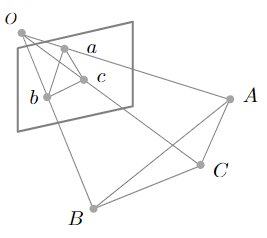
\includegraphics[width=0.38\textwidth]{Lec7/P3P}
    \caption{P3P}
\end{figure}

\begin{enumerate}
    \item 根据余弦定理
    \begin{align*}
        OA^{2}+OB^{2}-2 OA \cdot OB \cdot \cos \langle a, b\rangle=AB^{2} \\
        OB^{2}+OC^{2}-2 OB \cdot OC \cdot \cos \langle b, c\rangle=BC^{2} \\
        OA^{2}+OC^{2}-2 OA \cdot OC \cdot \cos \langle a, c\rangle=AC^{2}
    \end{align*}
    \item 同除$OC^2$, 令$x=\frac{OA}{OC}, y=\frac{OB}{OC}$
    \begin{align*}
        x^2+y^2-2xy\cos \langle a,b \rangle=\frac{AB^2}{OC^2}\\
        y^2+1^2-2xy\cos \langle b,c \rangle=\frac{BC^2}{OC^2}\\
        x^2+1^2-2xy\cos \langle a,c \rangle=\frac{AC^2}{OC^2}
    \end{align*}
    \item 令$v=\frac{AB^2}{OC^2}, u=\frac{BC^2}{AB^2}, w=\frac{AC^2}{AB^2}$
    \begin{align*}
        x^2+y^2-2xy\cos \langle a,b \rangle-v=0\\
        y^2+1^2-2xy\cos \langle b,c \rangle-uv=0\\
        x^2+1^2-2xy\cos \langle a,c \rangle-wv=0
    \end{align*}
    \item 消去$v$并重排, 得二元二次方程组
    \begin{align*}
        (1-u)y^2-ux^2-\cos \langle b,c \rangle y+2uxy \cos \langle a,b \rangle +1=0\\
        (1-w)x^2-wy^2-\cos \langle a,c \rangle x+2wxy \cos \langle a,b \rangle +1=0
    \end{align*}
    \begin{align*}
        \text{Known: }& \cos \langle a,b \rangle, \cos \langle b,c \rangle, \cos \langle a,c \rangle, u, w\\
        \text{Unknown: }& x, y 
    \end{align*}

    有四个解, 两个在正面, 两个在背面, 所以用额外一对点验证是哪一个解
\end{enumerate}

\subsubsection{PnP}
优化问题, 最小化 reprojection error (重投影误差)
\begin{align*}
    \min_{R,t}&\sum_i \left\| p_i-K(RP_i+t) \right\|^2\\
    p_i&\text{为 2D 点}\\
    K(RP_i+t)&\text{为 3D 对应 2D 的关系}
\end{align*}

使用P3P初始化, 用Gauss-Newton优化. 得到的解应该是最准确的. 

注: 
\begin{itemize}
    \item R必须正交, 或用轴角直接写出R(减少变量数, 且保证正交)
    \item 收敛解非全局最优解, 需要初始化
\end{itemize}

一个比较好的流程是用P3P的RANSAC, 然后最小化一下误差. 

\subsection{Object Pose Estimation}
已知2D, 3D点与2D旋转求3D相对相机的位置与旋转, 需找3D与2D对应关系. 可以直接手动定义关键点然后转化为关键点匹配问题, 后求PnP问题. 

\section{Structure from Motion(SfM)}
给多张图, 获得三维点云以及相机位姿. 

\subsection{Solving SfM}
\begin{enumerate}
    \item Assume intrinsic matrix K is known for each camera. (假设内参已知)
    \item Find a few reliable corresponding points. (寻找一些点到点的对应关系, 特征匹配)
    \item Find relative camera position $t$ and orientation $R$. (求解相机相对平移与旋转)
    \item Find 3D position of secne points. (三角化交点找到三维空间具体位置)
\end{enumerate}

\subsection{Epipolar geometry}
对极几何, 描述一3D点在不同2D视角下的几何关系, 通过此反求出视角. 
\begin{figure}[H]
    \centering
    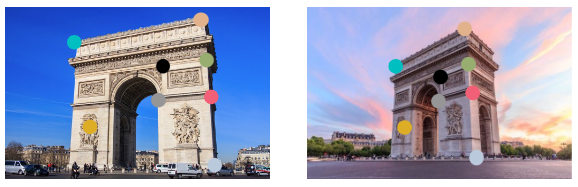
\includegraphics[width=0.68\textwidth]{Lec7/匹配}
    \caption{匹配}
\end{figure}

\begin{enumerate}
    \item base line(基线): the line connecting the center of cameras. (相机中心的连线)
    \item Epipole(极点): Image point of origin/pinhole of one camera as viewed by the other camera. (基线与相平面的角点) $e_l$与$e_r$为极点, 对每一对点, 其是唯一的. 
    \begin{figure}[H]
        \centering
        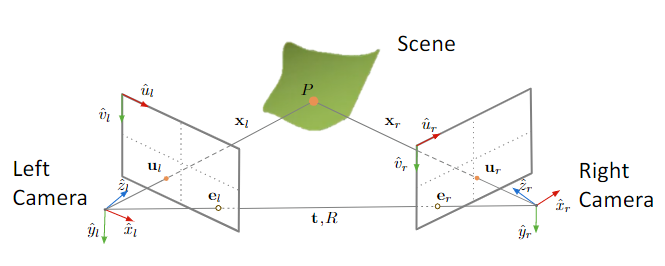
\includegraphics[width=0.58\textwidth]{Lec7/Epipolar geometry}
        \caption{Epipole}
    \end{figure}
    \item Epipolar Plane of Scene Point $P$: The plane formed by camera origins ($O_l$ and $O_r$), epipoles ($e_l$ and $e_r$) and scene point $P$. (相机中心与$P$构成的平面, 对每个$P$,其也是唯一的)
    \begin{figure}[H]
        \centering
        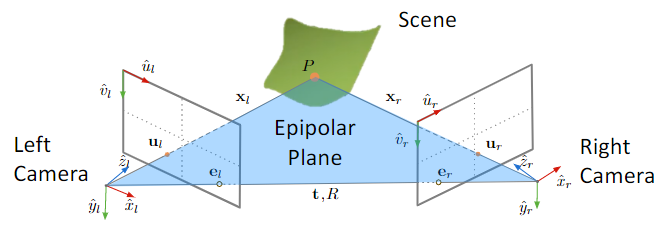
\includegraphics[width=0.58\textwidth]{Lec7/Epipolar Plane}
        \caption{Epipolar Plane}
    \end{figure}
\end{enumerate}

\subsubsection{Epipolar Constraint}
极线约束, 目的是描述$e_l$与$e_r$的关系. 
\begin{figure}[H]
    \centering
    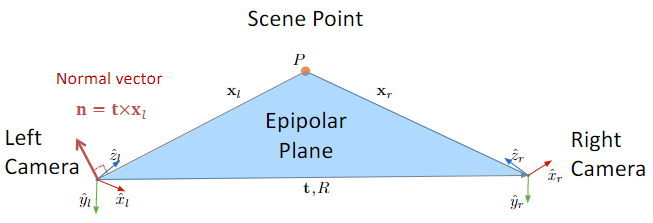
\includegraphics[width=0.58\textwidth]{Lec7/Epipolar Constraint}
    \caption{Epipolar Constraint}
\end{figure}

\begin{align*}
    \text{$P$相对于 Left Camera 的坐标: }&\vec{x}_l\\
    \text{$P$相对于 Right Camera 的坐标: }&\vec{x}_r\\
    \text{相机基线: }&\vec{t}\\
    \text{相机相对旋转: }&R\\
    \therefore \,  \text{极平面法向量: }&\vec{n}=\vec{t}\times \vec{x}_l\\
\end{align*}
\begin{align*}
    \therefore \,  \vec{x}_l \cdot (\vec{t}\times \vec{x}_l)&=0\\
    \begin{bmatrix}
        x_l&y_l&z_l
    \end{bmatrix}\begin{bmatrix}
        t_y z_l-t_z y_l\\
        t_z x_l-t_x z_l\\
        t_x y_l-t_y x_l\\
    \end{bmatrix}&=0\\
    \begin{bmatrix}
        x_l&y_l&z_l
    \end{bmatrix}
    \underset{T_{\times}}{\begin{bmatrix}
        0&-t_z&t_y\\
        t_z&0&-t_x\\
        -t_y&t_x&0
    \end{bmatrix}}
    \begin{bmatrix}
        x_l\\y_l\\z_l
    \end{bmatrix}
    &=0
\end{align*}

易知: 
\begin{align*}
    \vec{x}_l&=R\vec{x}_r+\vec{t}\\
    \begin{bmatrix}
        x_l\\y_l\\z_l
    \end{bmatrix}&=\begin{bmatrix}
        r_{11} & r_{12} & r_{13}\\
        r_{21} & r_{22} & r_{23}\\
        r_{31} & r_{32} & r_{33}
    \end{bmatrix}\begin{bmatrix}
        x_r\\y_r\\z_r
    \end{bmatrix}+\begin{bmatrix}
        t_x\\t_y\\t_z
    \end{bmatrix}
\end{align*}

代入得: 
\begin{align*}
    \begin{bmatrix}
        x_l&y_l&z_l
    \end{bmatrix}\left(\begin{bmatrix}
        0&-t_z&t_y\\
        t_z&0&-t_x\\
        -t_y&t_x&0
    \end{bmatrix}\begin{bmatrix}
        r_{11} & r_{12} & r_{13}\\
        r_{21} & r_{22} & r_{23}\\
        r_{31} & r_{32} & r_{33}
    \end{bmatrix}\begin{bmatrix}
        x_r\\y_r\\z_r
    \end{bmatrix}+
    \underset{T_{\times} \cdot \vec{t}=\vec{t}\times\vec{t}=0}{\begin{bmatrix}
        0&-t_z&t_y\\
        t_z&0&-t_x\\
        -t_y&t_x&0
    \end{bmatrix}\begin{bmatrix}
        t_x\\t_y\\t_z
    \end{bmatrix} }
    \right)&=0
\end{align*}
\begin{align*}
    \therefore \,  \begin{bmatrix}
        x_l&y_l&z_l
    \end{bmatrix}
    \underset{E}{\begin{bmatrix}
        e_{11} & e_{12} & e_{13} \\
        e_{21} & e_{22} & e_{23} \\
        e_{31} & e_{32} & e_{33}
    \end{bmatrix}}\begin{bmatrix}
        x_r\\y_r\\z_r
    \end{bmatrix}&=0\\
    \text{Essential Matrix(本质矩阵): }E=T_{\times}R
\end{align*}

The Decomposition (分解) of Essential Matrix $E$: 若$E$已知, 可以获得$\vec{t}$与$R$. (具体方法略去)

\subsubsection{Find Essential Matrix $E$}
\begin{align*}
    \vec{x}_l^T E \vec{x}_r=0
\end{align*}

但仅已知二维坐标, $\vec{x}_l$与$\vec{x}_r$未知. 但其可以使用二维坐标表示, 即透视变换. 
\begin{align*}
    z_{l}
    \begin{bmatrix}
        u_{l} \\
        v_{l} \\
        1
    \end{bmatrix}=\begin{bmatrix}
        z_{l} u_{l} \\
        z_{l} v_{l} \\
        z_{l}
    \end{bmatrix}=\begin{bmatrix}
        f_{x}^{(l)} x_{l}+z_{l} o_{x}^{(l)} \\
        f_{y}^{(l)} y_{l}+z_{l} o_{y}^{(l)} \\
        z_{l}
    \end{bmatrix}=
    \underset{\text{Camera Matirx }K_l}{\begin{bmatrix}
        f_{x}^{(l)} & 0 & o_{x}^{(l)} \\
        0 & f_{y}^{(l)} & o_{y}^{(l)} \\
        0 & 0 & 1
    \end{bmatrix}}\begin{bmatrix}
        x_{l} \\
        y_{l} \\
        z_{l}
    \end{bmatrix}
\end{align*}
\begin{align*}
    z_{l}
    \begin{bmatrix}
        u_{l} \\
        v_{l} \\
        1
    \end{bmatrix}&=\underset{K_l}{\begin{bmatrix}
        f_{x}^{(l)} & 0 & o_{x}^{(l)} \\
        0 & f_{y}^{(l)} & o_{y}^{(l)} \\
        0 & 0 & 1
    \end{bmatrix}}\begin{bmatrix}
        x_{l} \\
        y_{l} \\
        z_{l}
    \end{bmatrix}\\
    z_{r}
    \begin{bmatrix}
        u_{r} \\
        v_{r} \\
        1
    \end{bmatrix}&=\underset{K_r}{\begin{bmatrix}
        f_{x}^{(r)} & 0 & o_{x}^{(r)} \\
        0 & f_{y}^{(r)} & o_{y}^{(r)} \\
        0 & 0 & 1
    \end{bmatrix}}\begin{bmatrix}
        x_{r} \\
        y_{r} \\
        z_{r}
    \end{bmatrix}\\
    \therefore \,   \vec{x}_l^T&=\begin{bmatrix}
        u_l&v_l&1
    \end{bmatrix}z_l {K_l^{-1}}^T\\
    \vec{x}_r&=K_r^{-1} z_r \begin{bmatrix}
        u_{r} \\
        v_{r} \\
        1
    \end{bmatrix}
\end{align*}

由此得
\begin{align*}
    \begin{bmatrix}
        x_l&y_l&z_l
    \end{bmatrix}
    \begin{bmatrix}
        e_{11} & e_{12} & e_{13} \\
        e_{21} & e_{22} & e_{23} \\
        e_{31} & e_{32} & e_{33}
    \end{bmatrix}\begin{bmatrix}
        x_r\\y_r\\z_r
    \end{bmatrix}&=0\\
    \begin{bmatrix}
        u_l&v_l&1
    \end{bmatrix}z_l {K_l^{-1}}^T\begin{bmatrix}
        e_{11} & e_{12} & e_{13} \\
        e_{21} & e_{22} & e_{23} \\
        e_{31} & e_{32} & e_{33}
    \end{bmatrix}K_r^{-1} z_r \begin{bmatrix}
        u_{r} \\
        v_{r} \\
        1
    \end{bmatrix}&=0
\end{align*}

虽然$z_l$与$z_r$未知, 但因为右为0, 所以可以忽略, 得: 
\begin{align*}
    \begin{bmatrix}
        u_l&v_l&1
    \end{bmatrix}{K_l^{-1}}^T\begin{bmatrix}
        e_{11} & e_{12} & e_{13} \\
        e_{21} & e_{22} & e_{23} \\
        e_{31} & e_{32} & e_{33}
    \end{bmatrix}K_r^{-1}\begin{bmatrix}
        u_{r} \\
        v_{r} \\
        1
    \end{bmatrix}&=0\\
\end{align*}

令 $E=K_l^T F K_r$, 
\begin{align*}
    \therefore \, \begin{bmatrix}
        u_l&v_l&1
    \end{bmatrix}
    \underset{\text{Fundamental Matirx $F$}}{\begin{bmatrix}
        f_{11} & f_{12} & f_{13} \\
        f_{21} & f_{22} & f_{23} \\
        f_{31} & f_{32} & f_{33}
    \end{bmatrix}}\begin{bmatrix}
        u_{r} \\
        v_{r} \\
        1
    \end{bmatrix}&=0\\
\end{align*}

也有Scale的问题, 所以也需要$\|F\|=1$的约束. 

\subsection{Relative Camera Pose Estimation}
\begin{enumerate}
    \item For each correspondence $i$, write out epipolar constraint. 
    \begin{align*}
        \underset{\text{Known}}{\begin{bmatrix}
            u_{l}^{(i)} & v_{l}^{(i)} & 1
        \end{bmatrix}}
        \underset{\text{Unknown}}{\begin{bmatrix}
            f_{11} & f_{12} & f_{13} \\
            f_{21} & f_{22} & f_{23} \\
            f_{31} & f_{32} & f_{33}
        \end{bmatrix}}
        \underset{\text{Known}}{\begin{bmatrix}
            u_{r}^{(i)} \\
            v_{r}^{(i)} \\
            1
        \end{bmatrix}}=0
    \end{align*}

    Then expand the matrix to get linear equation: 
    \begin{align*}
        \left(f_{11} u_{r}^{(i)}+f_{12} v_{r}^{(i)}+f_{13}\right) u_{l}^{(i)}+\left(f_{21} u_{r}^{(i)}+f_{22} v_{r}^{(i)}+f_{23}\right) v_{l}^{(i)}+f_{31} u_{r}^{(i)}+f_{32} v_{r}^{(i)}+f_{33}=0
    \end{align*}
    \item Rearrange terms to form a linear system.
    \begin{align*}
        \begin{array}{cccc}
            \begin{bmatrix}
                u_{l}^{(1)} u_{r}^{(1)} & u_{l}^{(1)} v_{r}^{(1)} & u_{l}^{(1)} & v_{l}^{(1)} u_{r}^{(1)} & v_{l}^{(1)} v_{r}^{(1)} & v_{l}^{(1)} & u_{r}^{(1)} & v_{r}^{(1)} & 1 \\
                \vdots & \vdots & \vdots & \vdots & \vdots & \vdots & \vdots & \vdots & \vdots \\
                u_{l}^{(i)} u_{r}^{(i)} & u_{l}^{(i)} v_{r}^{(i)} & u_{l}^{(i)} & v_{l}^{(i)} u_{r}^{(i)} & v_{l}^{(i)} v_{r}^{(i)} & v_{l}^{(i)} & u_{l}^{(i)} & u_{r}^{(i)} & 1 \\
                \vdots & \vdots & \vdots & \vdots & \vdots & \vdots & \vdots & \vdots & \vdots \\
                u_{l}^{(m)} u_{r}^{(m)} & u_{l}^{(m)} v_{r}^{(m)} & u_{l}^{(m)} & v_{l}^{(m)} u_{r}^{(m)} & v_{l}^{(m)} v_{r}^{(m)} & v_{l}^{(m)} & u_{l}^{(m)} & u_{r}^{(m)} & 1
            \end{bmatrix}&\begin{bmatrix}
                f_{11}\\f_{12}\\f_{13}\\
                f_{21}\\f_{22}\\f_{23}\\
                f_{31}\\f_{32}\\f_{33}\\
            \end{bmatrix}&=&\begin{bmatrix}
                0\\0\\0\\
                0\\0\\0\\
                0\\0\\0\\
            \end{bmatrix}\\
            A&\vec{f}&\\
            \text{Known}&\text{Unknown}&
        \end{array}
    \end{align*}
    \begin{align*}
        A\vec{f}=0
    \end{align*}
    \item Find least squares solution for fundamental matrix $F$.
    \begin{align*}
        min_{\vec{f}}\left\| A\vec{f} \right\|,\text{ when }\left\| \vec{f} \right\|=1
    \end{align*}

    对$A^TA$使用特征值分解, 取其最小特征值对应特征向量就是我们的解. 

    Rearrange solution $\vec{f}$ to form the fundamental matrix $F$.
    \item Compute essential matrix $E$ from known left and right intrinsic camera matrices and fundamental matrix $F$.
    \begin{align*}
        E=k_l^T F K_r
    \end{align*}
    \item Extract $R$ and $\vec{t}$ from $E$.(Using Singular Value Decomposition)
    \begin{align*}
        E=T_{\times}R
    \end{align*}

\end{enumerate}

\subsection{Triangulation}
\begin{figure}[H]
    \centering
    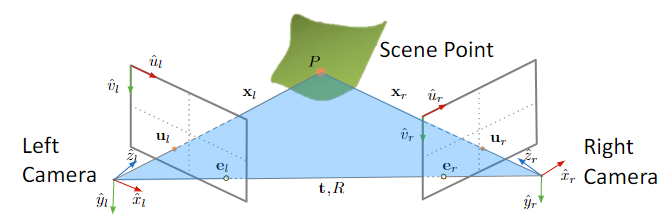
\includegraphics[width=0.68\textwidth]{Lec7/Triangulation}
    \caption{Triangulation}
\end{figure}

已知相机相对位姿与内参, 使用三角化测定三维的点位置. 

\begin{align*}
    \begin{bmatrix}
        u_{l} \\
        v_{l} \\
        1
    \end{bmatrix}&\equiv\begin{bmatrix}
        f_{x}^{(l)} & 0 & o_{x}^{(l)} & 0\\
        0 & f_{y}^{(l)} & o_{y}^{(l)} & 0\\
        0 & 0 & 1&0
    \end{bmatrix}\begin{bmatrix}
        x_{l} \\
        y_{l} \\
        z_{l} \\
        1
    \end{bmatrix}\\
    \begin{bmatrix}
        u_{r} \\
        v_{r} \\
        1
    \end{bmatrix}&\equiv\begin{bmatrix}
        f_{x}^{(r)} & 0 & o_{x}^{(r)} & 0\\
        0 & f_{y}^{(r)} & o_{y}^{(r)} & 0\\
        0 & 0 & 1 & 0
    \end{bmatrix}\begin{bmatrix}
        x_{r} \\
        y_{r} \\
        z_{r} \\
        1
    \end{bmatrix}\\
    \text{and}\,
    \begin{bmatrix}
        x_{l} \\
        y_{l} \\
        z_{l} \\
        1
    \end{bmatrix}
    &=\begin{bmatrix}
        r_{11} & r_{12} & r_{13} & t_x\\
        r_{21} & r_{22} & r_{23} & t_y\\
        r_{31} & r_{32} & r_{33} & t_z\\
        0&0&0&1
    \end{bmatrix}
    \begin{bmatrix}
        x_{r} \\
        y_{r} \\
        z_{r} \\
        1
    \end{bmatrix}
\end{align*}
\begin{align*}
    \therefore \, 
    \begin{bmatrix}
        u_{l} \\
        v_{l} \\
        1
    \end{bmatrix}&\equiv\begin{bmatrix}
        f_{x}^{(l)} & 0 & o_{x}^{(l)} & 0\\
        0 & f_{y}^{(l)} & o_{y}^{(l)} & 0\\
        0 & 0 & 1&0
    \end{bmatrix}\begin{bmatrix}
        r_{11} & r_{12} & r_{13} & t_x\\
        r_{21} & r_{22} & r_{23} & t_y\\
        r_{31} & r_{32} & r_{33} & t_z\\
        0&0&0&1
    \end{bmatrix}
    \begin{bmatrix}
        x_{r} \\
        y_{r} \\
        z_{r} \\
        1
    \end{bmatrix}\\
    \begin{bmatrix}
        u_{r} \\
        v_{r} \\
        1
    \end{bmatrix}&\equiv\begin{bmatrix}
        f_{x}^{(r)} & 0 & o_{x}^{(r)} & 0\\
        0 & f_{y}^{(r)} & o_{y}^{(r)} & 0\\
        0 & 0 & 1 & 0
    \end{bmatrix}\begin{bmatrix}
        x_{r} \\
        y_{r} \\
        z_{r} \\
        1
    \end{bmatrix}
\end{align*}
\begin{align*}
    \therefore \, \tilde{u}_l&=P_l\tilde{x}_r\\
    \tilde{u}_r&=M_{{int}_r}\tilde{x}_r\\
\end{align*}
\begin{align*}
    \therefore \,
    \begin{bmatrix}
        u_{r} \\
        v_{r} \\
        1
    \end{bmatrix}&\equiv\begin{bmatrix}
        m_{11} & m_{12} & m_{13} & m_{14} \\
        m_{21} & m_{22} & m_{23} & m_{24} \\
        m_{31} & m_{32} & m_{33} & m_{34}
    \end{bmatrix}\begin{bmatrix}
        x_{r} \\
        y_{r} \\
        z_{r} \\
        1
    \end{bmatrix}\\
    \begin{bmatrix}
        u_{r} \\
        v_{r} \\
        1
    \end{bmatrix}&\equiv\begin{bmatrix}
        p_{11} & p_{12} & p_{13} & p_{14} \\
        p_{21} & p_{22} & p_{23} & p_{24} \\
        p_{31} & p_{32} & p_{33} & p_{34}
    \end{bmatrix}\begin{bmatrix}
        x_{r} \\
        y_{r} \\
        z_{r} \\
        1
    \end{bmatrix}
\end{align*}

Rearranging the terms:
\begin{align*}
    \underset{A_{4\times3}}{\begin{bmatrix}
        u_{r} m_{31}-m_{11} & u_{r} m_{32}-m_{12} & u_{r} m_{33}-m_{13} \\
        v_{r} m_{31}-m_{21} & v_{r} m_{32}-m_{22} & v_{r} m_{33}-m_{23} \\
        u_{l} p_{31}-p_{11} & u_{l} p_{32}-p_{12} & u_{l} p_{33}-p_{13} \\
        v_{l} p_{31}-p_{21} & v_{l} p_{32}-p_{22} & v_{l} p_{33}-p_{23}
    \end{bmatrix}}
    \underset{\vec{x}_r}{\begin{bmatrix}
        x_{r} \\
        y_{r} \\
        z_{r}
    \end{bmatrix}}=
    \underset{\vec{b}_{4\times1}}{\begin{bmatrix}
        m_{14}-m_{34} \\
        m_{24}-m_{34} \\
        p_{14}-p_{34} \\
        p_{24}-p_{34}
    \end{bmatrix}}
\end{align*}

\begin{figure}[H]
    \centering
    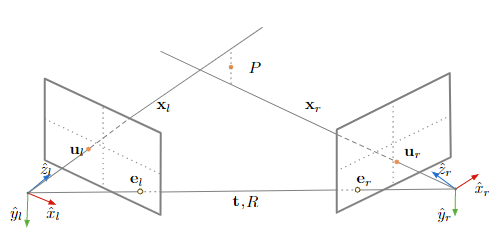
\includegraphics[width=0.58\textwidth]{Lec7/not exactly intersect}
    \caption{not exactly intersect}
\end{figure}

Generally, rays $x_l$ and $x_r$ will not exactly intersect. Find least squares solution by:
\begin{align*}
    \vec{x}_r=(A^TA)^{-1}A^T \vec{b}
\end{align*}

\begin{figure}[H]
    \centering
    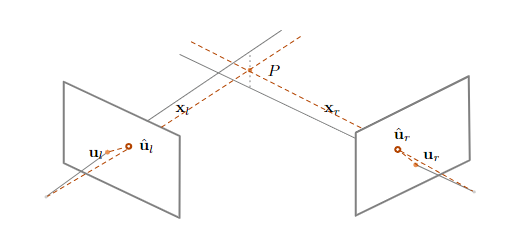
\includegraphics[width=0.58\textwidth]{Lec7/Minimize reprojection error}
    \caption{Minimize reprojection error}
\end{figure}

Or minimize reprojection error(重投影误差):
\begin{align*}
    cost(\mathrm{P})=\left\| \vec{u}_l-\hat{u}_l \right\|^2+\left\| \vec{u}_r-\hat{u}_r \right\|^2
\end{align*}

\subsection{Sequential Structure from Motion(Multi-frame structure from motion)}
序列式重建, 一帧一帧去建. 

\begin{enumerate}
    \item Initialize camera motion and scene structure. (前比较近的两帧先得到三维点云, 以第一帧做世界坐标系)
    \item For each additional view: 
    \begin{enumerate}
        \item Determine projection matrix of new camera using all the known 3D points that are visible in its image. (视觉定位估计新相机位姿)
        \item Refine and extend structure: compute new 3D points, reoptimize existing points that are also seen by this camera. (新增特征点三角化加入三维点云)
    \end{enumerate}
    \item Refine structure and motion: Bundle Adjustment.(集束调整, 后处理) 
    
    \begin{figure}[H]
        \centering
        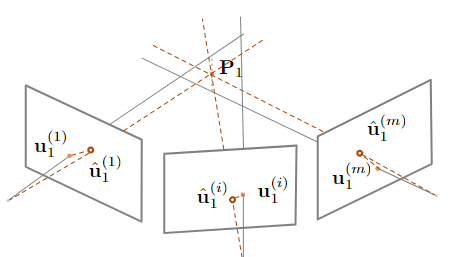
\includegraphics[width=0.48\textwidth]{Lec7/Bundle adjustment}
        \caption{Bundle adjustment}
    \end{figure}

    Refining 3D points and camera parameters by minimizing reprojection error over all frames.(最小化所有点的重投影误差并优化相机位姿, m帧, n关键点)
    \begin{align*}
        E(P_{proj},\vec{P})=\sum_{i=1}^m \sum_{j=1}^n \left\| u_j^{(i)}-P_{proj}^{(i)}\vec{P}_j \right\|^2
    \end{align*}
\end{enumerate}